\documentclass[a4paper,10pt]{article}

%\usepackage[a4paper]{geometry}
\usepackage{fullpage}
\usepackage{graphicx}
\usepackage{graphics}
\usepackage{wrapfig}
\usepackage{paralist}
\usepackage{color}


\title{DMML Coursework 1}
\author{Joseph Davidson - 071729468}
\date{}

\begin{document}

  \maketitle

  \section{Introduction}
    This is the coursework submission from Joseph Davidson for the DMML
    coursework 1. The tools I used for this coursework were: awk (for all the
    processing, finding accuracy of 1-NN, creating the raw chart data),
    Google Docs for creating the charts and \LaTeX{} for making this pretty 
    report that you're currently reading. Vim was the editor of choice.

  \section{Accuracy of 1-NN}

    The results are presented in the table below:

    \begin{table}[hc]
      \centering
      \caption{Accuracy in \% of 1-NN normalized vs non-normalized.} \indent
      \begin{tabular}{|c|c|c|}
        \hline
                      & \textbf{Non-Normalized} & \textbf{Normalized} \\ \hline
        Comm + Crime  &                  &              \\ 
        Yeast         &                  &              \\
        Pima Indians  &                  &              \\ 
        Authors       &                  &              \\
        \hline
      \end{tabular}
    \end{table}
    As can be seen, the normalization of the data increases the accuracy of 1-NN. This is
    especially visible in the ``Authors" data set. Which indicates that the normalization process
    has greatly exemplified the writing style of the two authors allowing 1-NN to classify the data
    much more accurately.
    The Communities and Crime dataset really didn't have much of a difference before an after its Z-normalization.
    This is probably because Z-normalizing tries to transform the input such that the mean is as close to 0 as
    possible while the standard deviation are close to 1. The original max-min normalized values of the dataset
    are quite close to 0 anyway, so the Z-normalization didn't have as much of an effect as it could have.
    The Yeast dataset had only a small increase too, this is because the normalized values differ only very
    slightly from the original values $*100$. It appears to me that normalization techniques only have much
    of an effect when they significantly change the data in the set (as is the case with the Authors dataset). 

    \section{Histograms}
      The histograms for the 4 datasets are presented below.
      We will see the histograms for the first 5 fields of: 
      \begin{inparaenum}[(1)]
        \item the Yeast Dataset
        \item Pima Indians Diabetes Dataset
        \item Authors Dataset and
        \item the Communities and Crime Dataset.
      \end{inparaenum}
       and each page will hold a brief discussion on differences of the class fields and the suitability
       of the 5 fields for effectively classifying instances. Each of the datasets have been converted to 
       2-class and are all min-max normalized. The 5-bin distribution is from 1 to 100, so there are obvious
       values for each bin.
                                                  
       \newpage
        \subsection{Yeast Dataset Histograms}

        \begin{figure}[ht!]
          \begin{minipage}[b]{0.5\linewidth}
            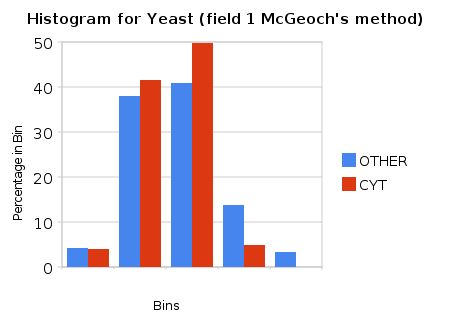
\includegraphics[scale=0.45]{charts/YeastPics/Y1.png}
          \end{minipage}
          \begin{minipage}[b]{0.5\linewidth}
             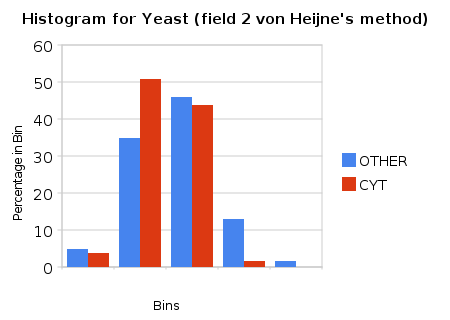
\includegraphics[scale=0.45]{charts/YeastPics/Y2.png}
          \end{minipage} 
        \end{figure}

        \begin{figure}[ht!]
          \begin{minipage}[b]{0.5\linewidth}
            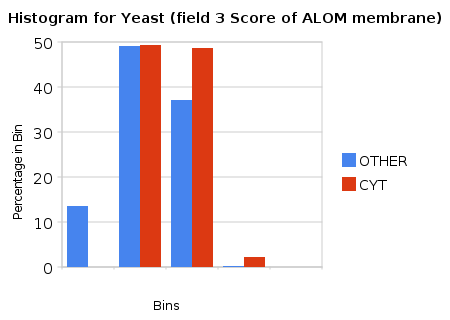
\includegraphics[scale=0.45]{charts/YeastPics/Y3.png}
          \end{minipage}
          \begin{minipage}[b]{0.5\linewidth}
             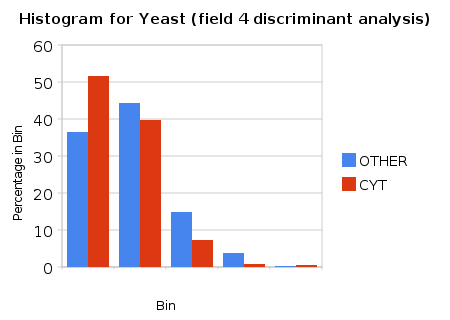
\includegraphics[scale=0.45]{charts/YeastPics/Y4.png}
          \end{minipage}
        \end{figure}

        \begin{figure}[ht!]
          \begin{minipage}[t]{0.5\linewidth}
              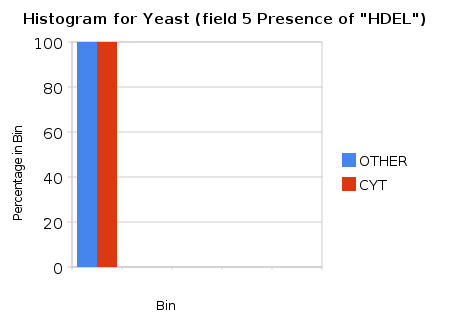
\includegraphics[scale=0.45]{charts/YeastPics/Y5.png}
          \end{minipage}
          \parbox[b]{3.5in}{
            These histograms are for the yeast dataset. In F1 we see that very high scores are not in class CYT
            and that scores that are in the middle bin tend to correlate more to CYT. Lower scores are about equal
            between CYT and OTHER yeasts.
            F2 also shows that higher scores are not CYT. Scores just below the median tend to be a lot more likely to 
            be CYT, whereas median scores have not much difference between them.
            F3 shows that median--higher scores are more likely to be CYT and that a very low score is not CYT. There is
            a roughly equal probability that the the yeast is CYT or not when the score is just below the median.
            In F4 we see that very low scores are more likely to be CYT, but otherwise there is not much to distinguish
            between the two.
            F5 has no use at all in this context, both CYT and others have HDEL in them. If this were a multi-class set,
            this field may help narrow down the possible class range (some yeasts in the ``OTHER" category may not have
            HDEL in them). But as HDEL is binary (you either have it, or you don't), it doesn't much distinguish in this
            context.
            The two fields I have chosen for the next part of the coursework is F1 and F3. This is because the two fields
            appear to show the greatest cumulative difference between the two classes. Hopefully, the next results will
            not be too severely impacted by the usage of only two fields by using these ones.    
          }
        \end{figure}
 
        \newpage
        \subsection{Pima Indians Diabetes Dataset}
 
        \begin{figure}[ht!]
          \begin{minipage}[b]{0.5\linewidth}
            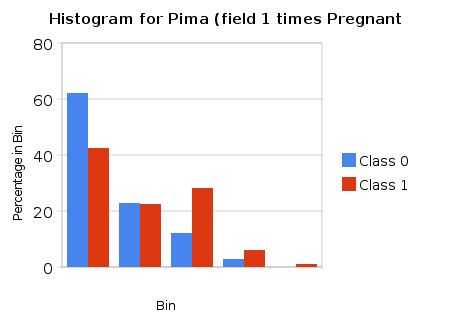
\includegraphics[scale=0.45]{charts/PimaPics/P1.png}
          \end{minipage}
          \begin{minipage}[b]{0.5\linewidth}
             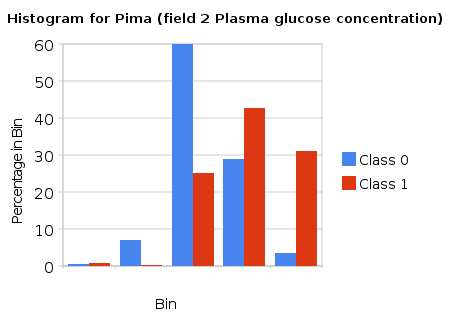
\includegraphics[scale=0.45]{charts/PimaPics/P2.png}
          \end{minipage}
        \end{figure}

        \begin{figure}[ht!]
          \begin{minipage}[b]{0.5\linewidth}
            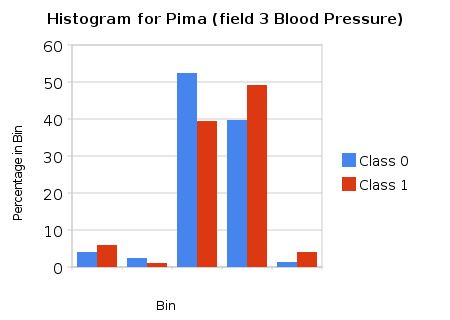
\includegraphics[scale=0.45]{charts/PimaPics/P3.png}
          \end{minipage}
          \begin{minipage}[b]{0.5\linewidth}
             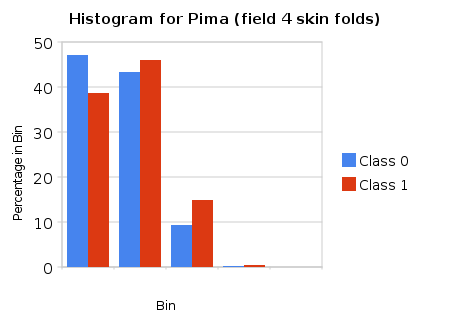
\includegraphics[scale=0.45]{charts/PimaPics/P4.png}
          \end{minipage}
        \end{figure}
        \begin{figure}[ht!]
          \begin{minipage}[t]{0.5\linewidth}
              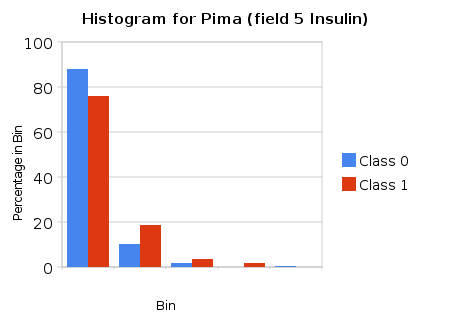
\includegraphics[scale=0.45]{charts/PimaPics/P5.png}
          \end{minipage}
          \parbox[b]{3.5in}{
             These histograms are for the Pima Indians Diabetes dataset. F1 indicates that those with more
             pregnancies are at a higher risk of diabetes. Naturally, this implies that men are at a lower risk
             of pregnancy related diabetes. F2 shows that a median--low blood glucose content indicates lower 
             risk, but that risk increased sharply when it is above the median. F3 implies that a median--low bp             
             generally indicates lower risk, but a higher bp increases the chance of developing diabetes. F4 has 
             no real correlation between the thickness of the skin folds on the Triceps whether the person has diabetes --
             I wouldn't have really expected there to be one. F5 shows that most of the sample group, diabetes or no,
             metabolised the provided insulin after 2 hours. Those with a level greater than the mean usually had
             diabetes though. The two fields I am going to choose for the next part of the coursework are F1 and F2
             because median--low scores in F2 mean that there is an increased chance that the subject doesn't have
             diabetes -- therefore easier classification. F1 shows a clear separation in probabilities between
             low--below Median and median--high pregnancies and their respective risks of diabetes.     
          }
        \end{figure}

        \newpage

        \subsection{Authors Dataset Histograms}

        \begin{figure}[ht!]
          \begin{minipage}[b]{0.5\linewidth}
            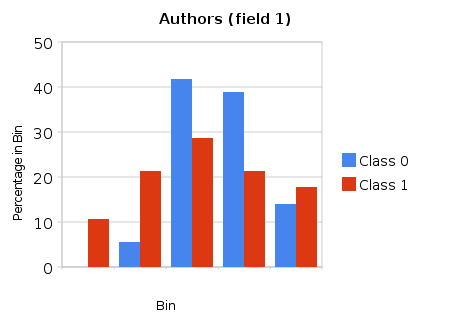
\includegraphics[scale=0.45]{charts/AuthorsPics/A1.png}
          \end{minipage}
          \begin{minipage}[b]{0.5\linewidth}
             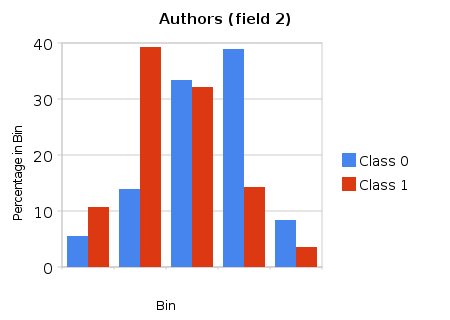
\includegraphics[scale=0.45]{charts/AuthorsPics/A2.png}
          \end{minipage}
        \end{figure}

        \begin{figure}[ht!]
          \begin{minipage}[b]{0.5\linewidth}
            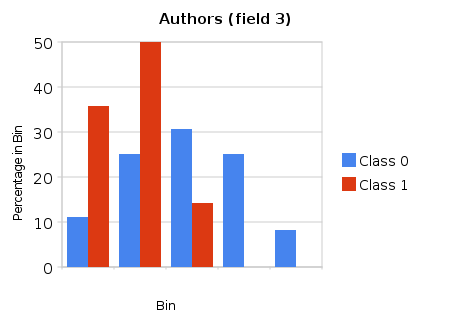
\includegraphics[scale=0.45]{charts/AuthorsPics/A3.png}
          \end{minipage}
          \begin{minipage}[b]{0.5\linewidth}
             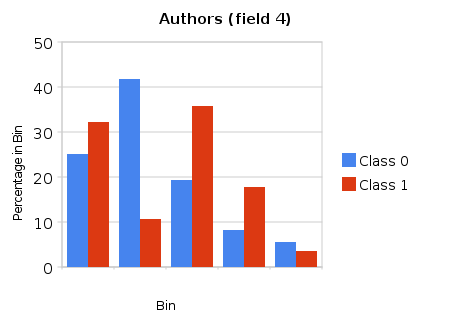
\includegraphics[scale=0.45]{charts/AuthorsPics/A4.png}
          \end{minipage}
        \end{figure}

        \begin{figure}[ht!]
          \begin{minipage}[t]{0.5\linewidth}
              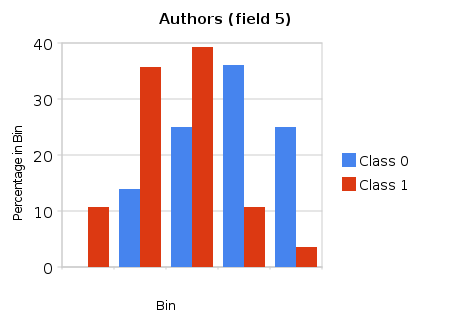
\includegraphics[scale=0.45]{charts/AuthorsPics/A5.png}
          \end{minipage}
          \parbox[b]{3.5in}{
            These histograms are for the Authors dataset. F1 shows that when word1 is used moderately, it indicates author 0
            whereas, when used sparsely or heavily, author 1 is likely to be the writer. F2 appears to be almost an exact
            mirror image of itself -- I don't quite get the significance of this (if any) though\ldots It shows that
            when word2 is used moderately, either author could have penned the text, but when it is used heavily or sparsely
            the chances of it being written by author 0 or author 1 respectively increases substantially. F3 shows that
            lower usage of word3 can be attributed to author 1, but author 0 almost exclusively uses word3 frequently in his
            texts. F4 shows that author 0 usually uses word4 at a frequency that is just below the median, but higher uses of
            word4 are in the style of author 1. With F5, it appears that median-low usage of word5 can be attributed to 
            author 1 but any usage more frequent than that indicates that author 0 wrote the text. It seems that there is
            nor really bad choice in selecting a couple of fields to go on with, but the two I've settled on are F3 and F5.
            F3 and F5 show a clear disparity between the two writers in their usage of words 3 and 5 respectively.   
          }
        \end{figure}

        \newpage
 
        \subsection{Communities and Crime Dataset Histograms}

        \begin{figure}[ht!]
          \begin{minipage}[b]{0.5\linewidth}
            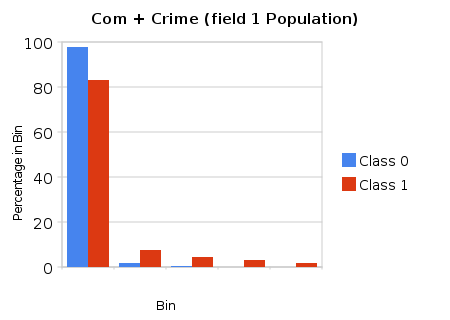
\includegraphics[scale=0.45]{charts/ComCrimePics/CC1.png}
          \end{minipage}
          \begin{minipage}[b]{0.5\linewidth}
             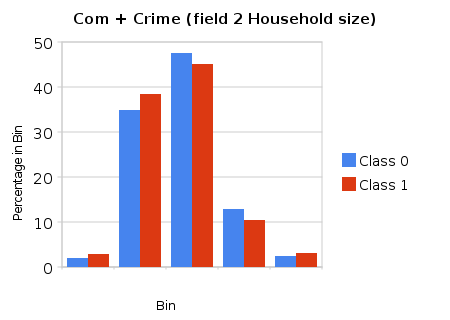
\includegraphics[scale=0.45]{charts/ComCrimePics/CC2.png}
          \end{minipage}
        \end{figure}

        \begin{figure}[ht!]
          \begin{minipage}[b]{0.5\linewidth}
            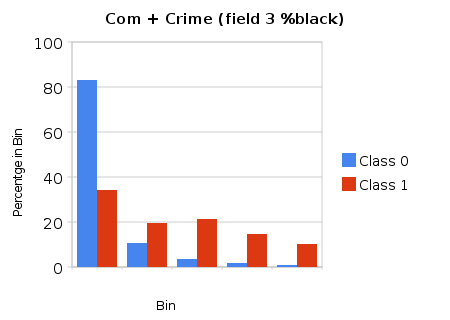
\includegraphics[scale=0.45]{charts/ComCrimePics/CC3.png}
          \end{minipage}
          \begin{minipage}[b]{0.5\linewidth}
             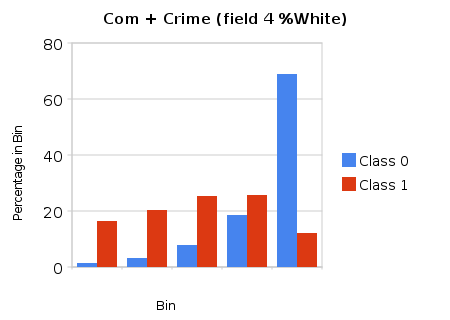
\includegraphics[scale=0.45]{charts/ComCrimePics/CC4.png}
          \end{minipage}
        \end{figure}

        \begin{figure}[ht!]
          \begin{minipage}[b]{0.5\linewidth}
              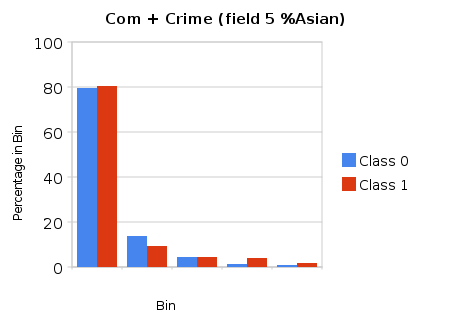
\includegraphics[scale=0.45]{charts/ComCrimePics/CC5.png}
          \end{minipage}
          \parbox[b]{3.5in}{
            F1 indicates that communities with lower
            populations overwhelmingly have both more petty and violent crime than anywhere else. Larger communities
            have a lot less of both, but the violent crime outweighs the petty crime. F2 doesn't show much distinction
            between communities with varying household sizes.
            F3 shows that communities with a low \%age of black people experience overwhelmingly more petty crime than
            those with a higher \%age. The violent crime tends to be around the same in the communities. With slightly more
            in low \%age communities than high \%age ones. F4 shows that communities with a higher \%age of white people
            have significantly more petty crime than communities with lower \%ages. The violent crime drops off at that point
            also, but communities with slightly less white people have more violent crime than comparable communities. F5 is
            rather interesting, it appears that as the \%age of Asian people in a community increases, crime tends to  drop
            off all together! Communities with a low \%age of Asian people have a very high petty and violent
            crime rate though. The chosen fields for the next part of the coursework are F3 and F4. This is because of the
            distinguish-ability of the classes within the fields, which will hopefully make classifying using 1-NN easier. 
          }
        \end{figure}
        \newpage

  \section{Accuracy of 1-NN on Two Fields}
    Here are the results for 1-NN using only 2 fields. They are quite interesting, red coloured results
    are less accurate than using 1-NN on entire records, whilst green results are more accurate.
    \begin{table}[hc]
      \centering
      \caption{Accuracy in \% of 1-NN on two fields normalized vs non-normalized.} \indent
      \begin{tabular}{|c|c|c|c|}
        \hline
                      &  \textbf{Fields Used}  & \textbf{Non-Normalized} & \textbf{Normalized} \\ \hline
        Comm + Crime  &   F3 \& F4       &   \textcolor{red}{}        &  \textcolor{green}{}    \\
        Yeast         &   F1 \& F3       &   \textcolor{red}{}        &  \textcolor{red}{}    \\
        Pima Indians  &   F1 \& F2       &   \textcolor{green}{}       &  \textcolor{green}{}    \\
        Authors       &   F3 \& F5       &   \textcolor{green}{}      &   \textcolor{red}{}    \\
        \hline
      \end{tabular}
    \end{table}
 
    Much to my surprise, it seems as though reducing the dataset actually increased the accuracy in some cases!
    In the case of the Pima Indians diabetes; less -- but more specific -- fields increased the accuracy of 1-NN
    in both the normalized and non-normalized cases. For others, it helped only one or the other and even in the
    case of Yeast: not at all.

  \section{Extra}
    In light of this extra space I have (and my desire for extra marks), I will compare the results from 3-NN to 1-NN and see what kind of
    improvement can be gleaned. The colouring scheme is as above with respect to the first table.
  
    \begin{table}[hc]
      \centering
      \caption{Accuracy in \% of 3-NN  normalized vs non-normalized.} 
      \begin{tabular}{|c|c|c|}
        \hline
                      & \textbf{Non-Normalized} & \textbf{Normalized} \\ \hline
        Comm + Crime  &   \textcolor{red}{19.2578}        &  \textcolor{red}{19.2578}    \\
        Yeast         &   \textcolor{green}{68.8008}      &  \textcolor{green}{68.8008}    \\
        Pima Indians  &   \textcolor{red}{34.6354}        &  \textcolor{red}{34.6354}    \\
        Authors       &   \textcolor{green}{56.9231}      &   \textcolor{red}{56.9231}    \\
        \hline
      \end{tabular}
    \end{table}
    Immediately apparent is that 3-NN completely negates the effects of normalization! The results are the same
    whether the input has been normalized or not. I also would have expected a large bump in the accuracy of the 
    classification for all the datasets. It seems that 3-NN typically performs \emph{worse} (if we take these datasets as a
    sampling of all datasets) than 1-NN! I would like to investigate further, but alas, I have other work that requires my
    attention. Hopefully this addendum earns me at least a modest amount of extra marks.


\end{document}
